\section{Operating Basics}

\subsection{Prepare your AXIOM Beta for use}

\begin{center}
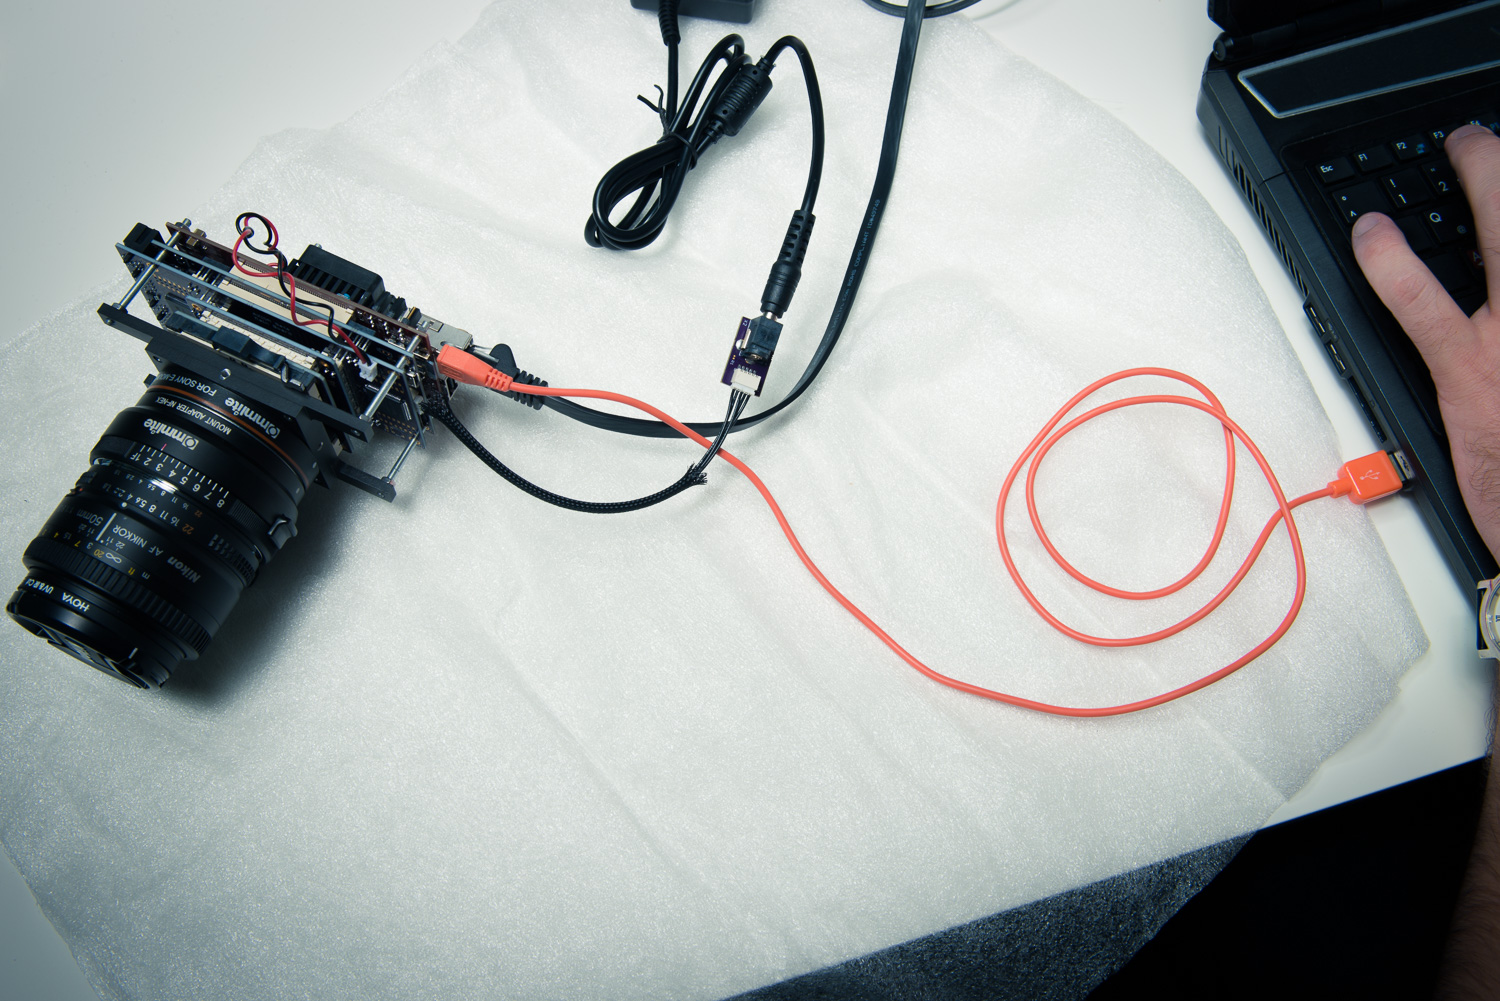
\includegraphics[height=11cm]{images/Getting_Started}\\
\end{center}

1. Use a micro-USB cable to connect the camera's MicroZed development board (USB UART) to a computer. The MicroZed board is the backmost, red PCB. (There is another micro-USB socket on the Power Board, but that is the JTAG Interface.)\\

2. Connect the ethernet port on the MicroZed to an ethernet port on your computer. You might have to use an ethernet adapter on newer, smaller machines which come without a native ethernet port.\\ 

3. Connect the AC adapter to the camera's Power Board. (The power cord plugs into an adapter that connects to the Power Board; to power the camera off at a later point, you need not disconnect the adapter from the board but can just unplug the cord from the adapter.)


\begin{center}
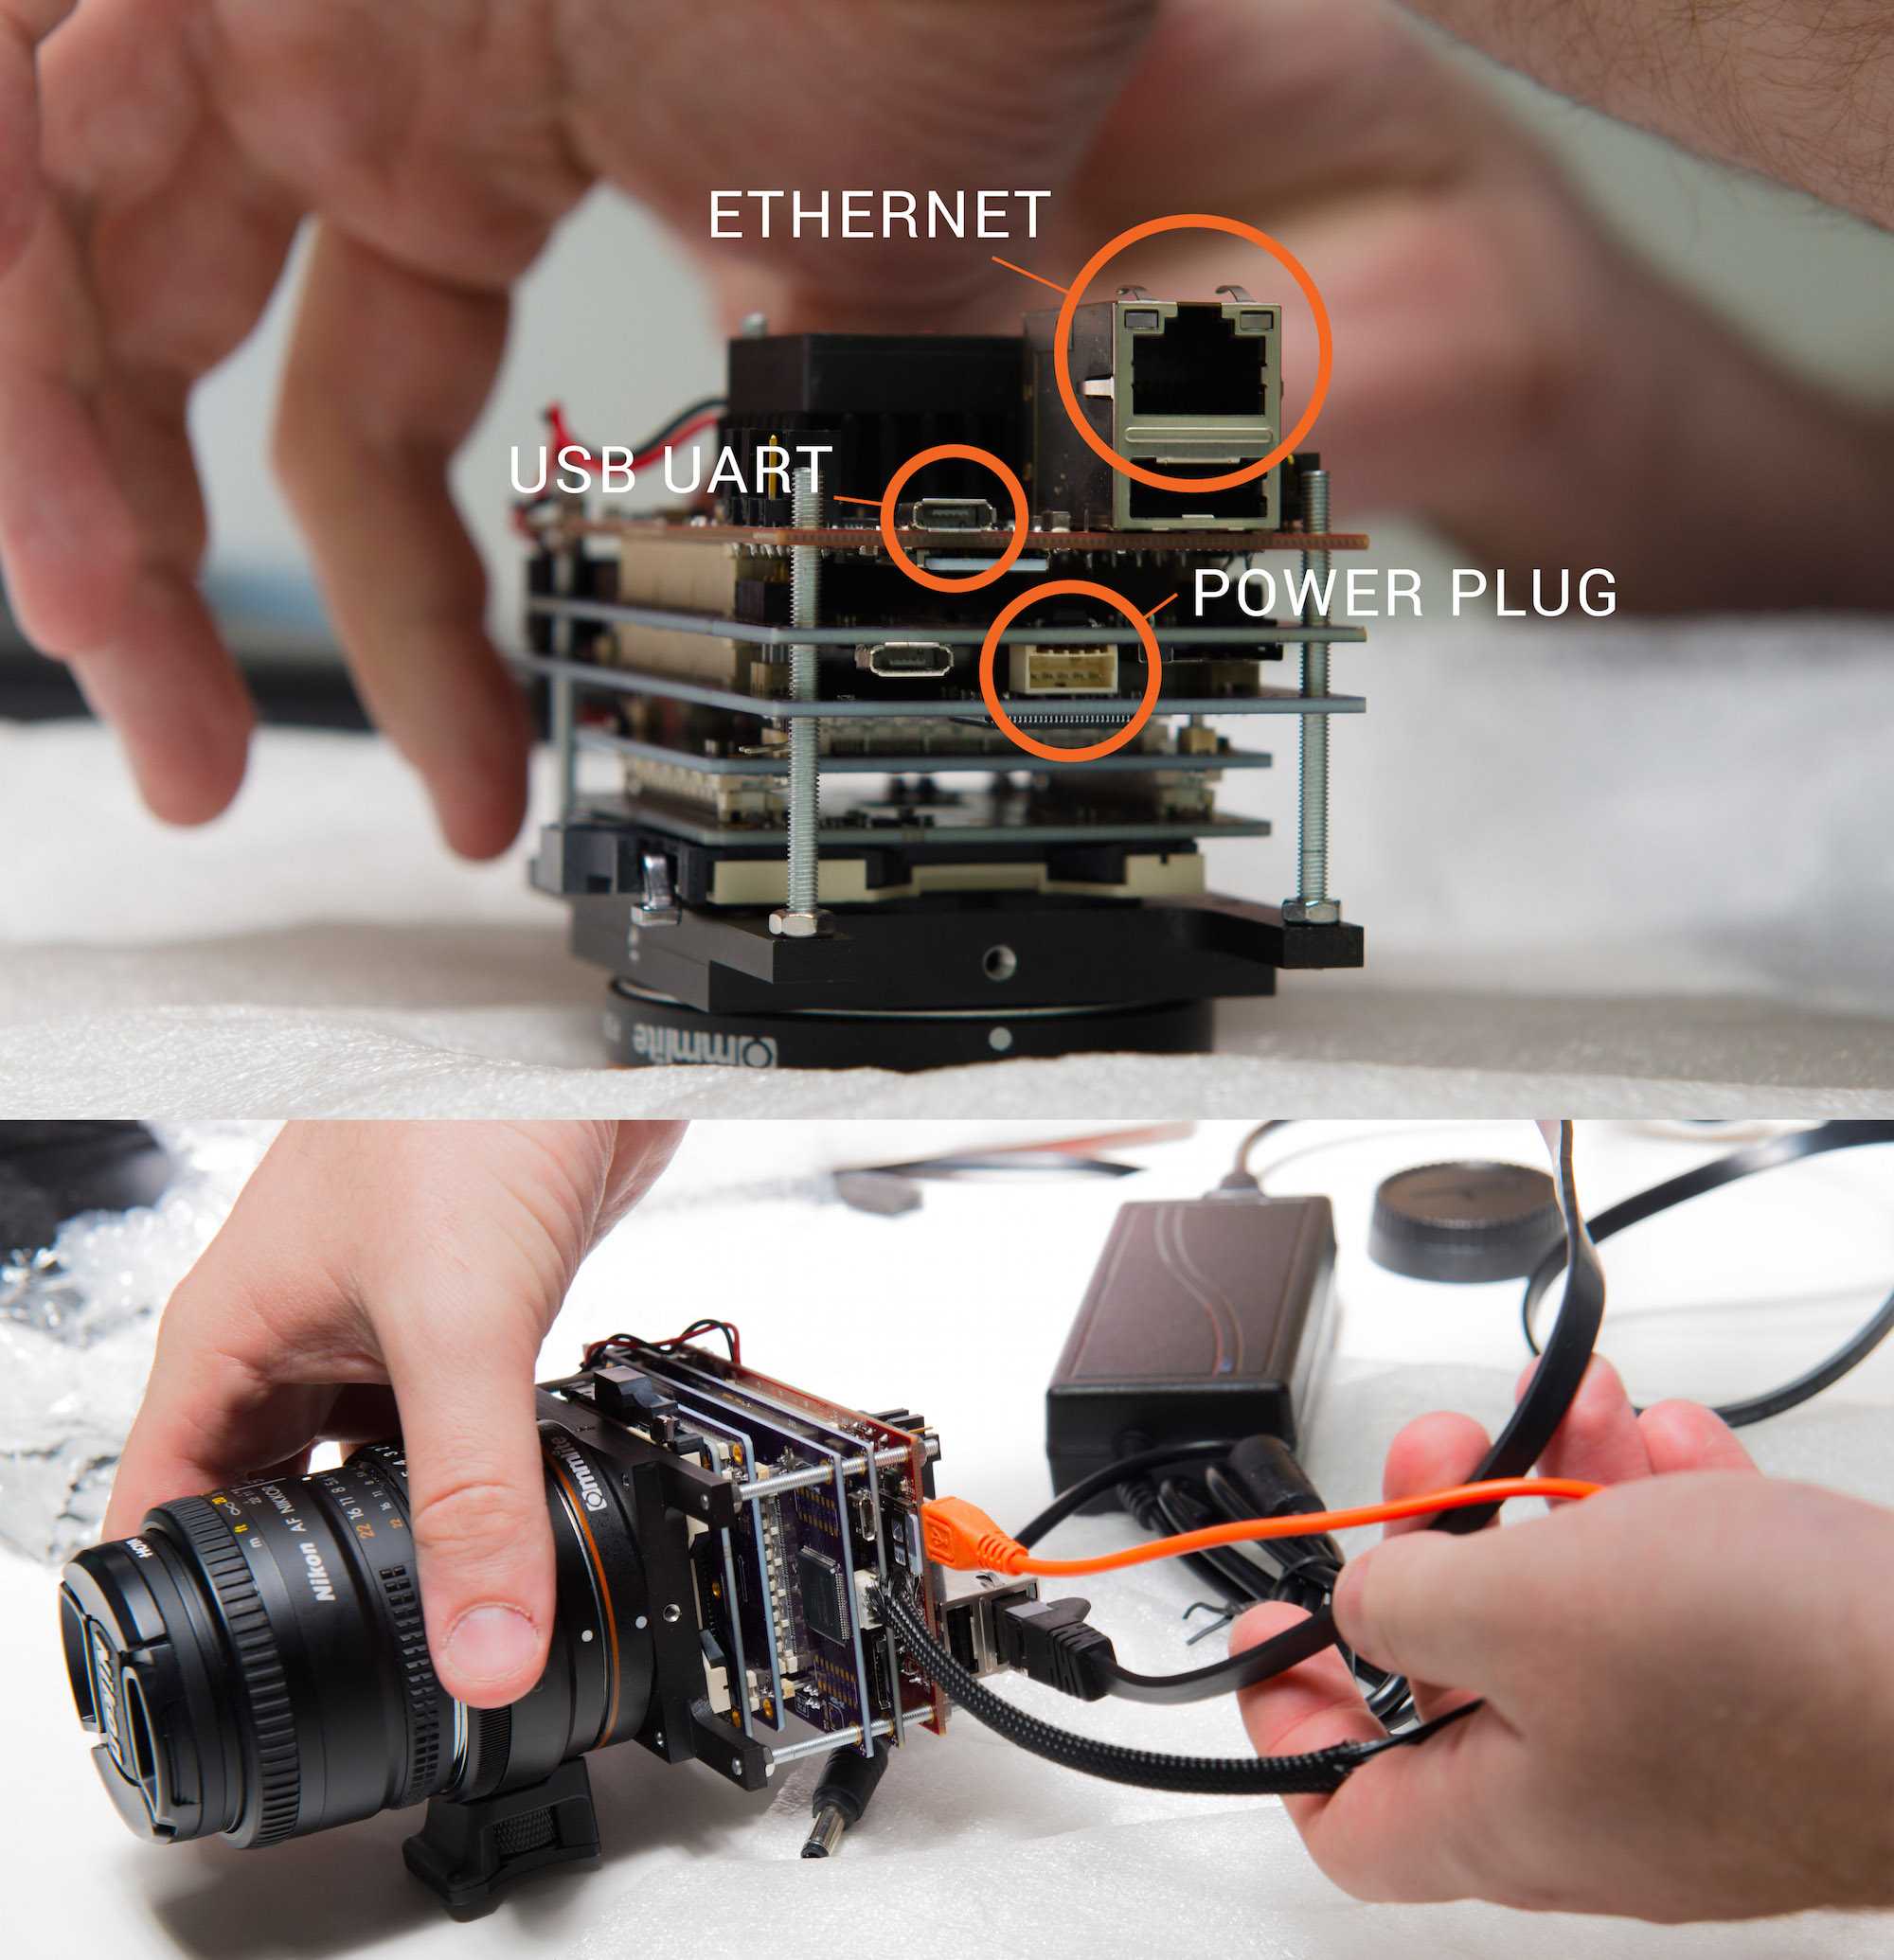
\includegraphics[height=17cm]{images/BetaGuide}\\
\end{center}

\subsection{Prepare your computer for use with AXIOM Beta}

\textbf{Overview -} To communicate with your AXIOM Beta camera, you will send it instructions via your computer's command line.\\

In case you have not worked with a shell (console, terminal) much or ever before, we have prepared detailed instructions to help you get you set up. The steps which need to 	be taken to prepare your machine sometimes differ between operating systems, so pick the ones that are applicable to you(r system). \\

\textbf{Note:} Dollar signs placed in front of commands are not meant to be typed in but denote the command line prompt (a signal indicating the computer is ready for user input). It is used in documentation to differentiate between commands and output resulting from commands. The prompt might look different on your machine (e.g. an angled bracket >) and be preceded by your user name, computer name or the name of the directory which you are currently inside.



\subsubsection{USB to UART Drivers}

For the USB connection to work, you will need drivers for bridging USB to UART (USB to serial). (Under Linux this works out of the box in most 	distributions) for other operating systems they can be \href{https://www.silabs.com/products/development-tools/software/usb-to-uart-bridge-vcp-drivers}{downloaded} from e.g. Silicon Labs' website – pick the software provided for your OS and install it. \\

\subsubsection{Serial Console}

The tool we recommend for connecting to the AXIOM Beta camera via serial port with Mac OS X or Linux is \href{https://linux.die.net/man/1/minicom}{minicom}; for connections from Windows machines, we have used \href{http://www.putty.org/}{Putty}.

\paragraph{Linux Setup}

Check if you already have minicom installed on your system by trying to run it:

\begin{lstlisting}[language=bash,morekeywords=$,keywordstyle=\bfseries,frame=none,xleftmargin=.25in,belowskip=2em, aboveskip=2em]
$ minicom
\end{lstlisting}

Your system will respond with a message like bash: command not found: minicom if it's not installed.





\paragraph{MAC OSX Setup}
\paragraph{Minicom Configuration}
\subsubsection{Serial connection (via USB)}
\paragraph{Connect using Minicom}\mbox{}\\
Note that you will not be able to use the terminal window you initiate the serial connection in for anything else (it needs to remain open while you access the camera), so it might make sense to open a separate window just for this purpose.

With minicom installed and properly configured, all you need to do is run the following command to start it with the correct settings:

\begin{lstlisting}[language=bash,morekeywords=$,keywordstyle=\bfseries,frame=none,xleftmargin=.25in,belowskip=2em, aboveskip=2em]
$ minicom -8 USB0
\end{lstlisting}

On successful connection, you will be prompted to enter user credentials (which are needed to log into the camera).\\

Test\\

If your terminal remains blank except for the minicom welcome screen/information about your connection settings, try pressing enter. If this still does not result in the prompt for user credentials – while testing, we discovered the initial connection with minicom does not always work – disconnect the camera from the power adapter, then reconnect it: in your minicom window you should now see the camera's operating system booting up, followed by the login prompt. (From then on, connecting with minicom should work smoothly and at most require you to press enter to make the login prompt appear.)

\paragraph{Connect using Screen}
\paragraph{Disconnect}
\subsubsection{Ethernet connection (using SSH)}
\paragraph{SSH Keys how-to for Linux and Mac}
\subparagraph{Storage location/Find existing keys}
\subparagraph{SSH key creation}
\paragraph{Get or set IP address}
\paragraph{IP address check}
\paragraph{Set IP address}
\paragraph{Establish a connection via key}
\paragraph{Password-based authentication}
\subsubsection{Start the camera}
\subsubsection{WiFi access point setup}
